\documentclass[12pt]{article}
\usepackage{bigints}
\usepackage{graphicx}			% Use this package to include images
\usepackage{amsmath}	
\usepackage{amssymb}
\usepackage{amsfonts}
\usepackage{polynom}
\usepackage{listings}
% A library of many standard math expressions
\graphicspath{ {./Images/} }
\usepackage[margin=1in]{geometry}% Sets 1in margins. 
\newcommand{\qed}[0]{$\blacksquare$}
\usepackage{fancyhdr}			% Creates headers and footers
\usepackage{enumerate}          %These two package give custom labels to a list
\usepackage[shortlabels]{enumitem}


% Creates the header and footer. You can adjust the look and feel of these here.
\pagestyle{fancy}
\fancyhead[l]{Aditya Gupta}
\fancyhead[c]{Amath Homework \#2}
\fancyhead[r]{\today}
\fancyfoot[c]{\thepage}
\renewcommand{\headrulewidth}{0.2pt} %Creates a horizontal line underneath the header
\setlength{\headheight}{15pt} %Sets enough space for the header
\begin{document}
1. 
\begin{figure}[h]
    \centering
    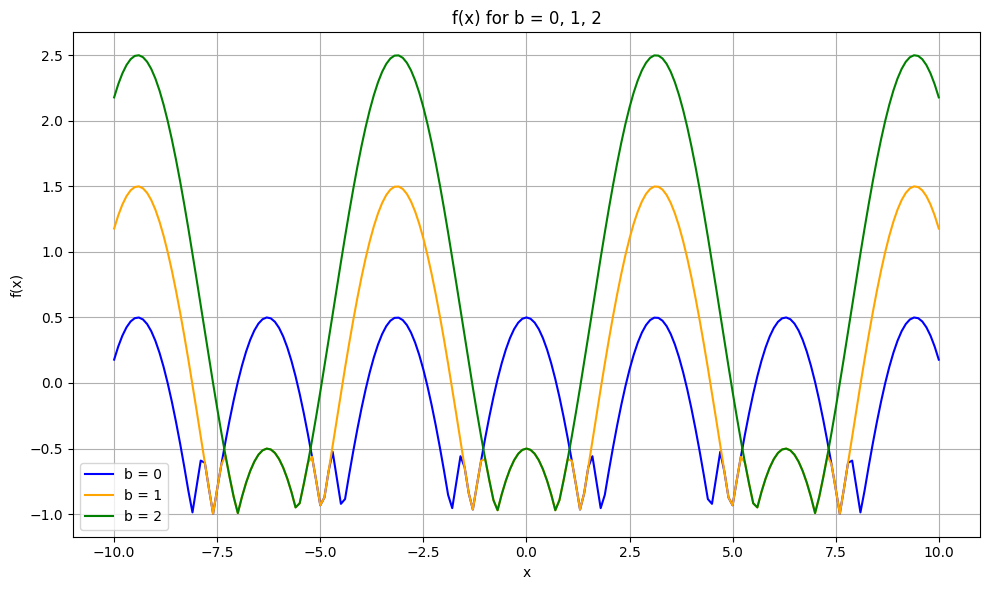
\includegraphics[width=0.75\linewidth]{AMath301/image.png}
\end{figure}
\begin{enumerate}




\item [2. ] The Taylor series approximation of \( f(x) = \cos(x) \), centered at \( x = 0 \), is given by:
\[
T_n(x) = \sum_{k=0}^n \frac{(-1)^k}{(2k)!} x^{2k}.
\]

Explicitly, the Taylor polynomials are:

1. For \( T_0(x) \) (polynomial of degree \( 2 \cdot 0 = 0 \)):
\[
T_0(x) = \frac{(-1)^0}{(2 \cdot 0)!} x^{2 \cdot 0} = 1.
\]

2. For \( T_2(x) \) (polynomial of degree \( 2 \cdot 2 = 4 \)):
\[
T_2(x) = \frac{(-1)^0}{(2 \cdot 0)!} x^{2 \cdot 0} 
+ \frac{(-1)^1}{(2 \cdot 1)!} x^{2 \cdot 1}
+ \frac{(-1)^2}{(2 \cdot 2)!} x^{2 \cdot 2}.
\]
\[
T_2(x) = 1 - \frac{x^2}{2!} + \frac{x^4}{4!}.
\]

3. For \( T_4(x) \) (polynomial of degree \( 2 \cdot 4 = 8 \)):
\[
T_4(x) = \frac{(-1)^0}{(2 \cdot 0)!} x^{2 \cdot 0} 
+ \frac{(-1)^1}{(2 \cdot 1)!} x^{2 \cdot 1}
+ \frac{(-1)^2}{(2 \cdot 2)!} x^{2 \cdot 2}
+ \frac{(-1)^3}{(2 \cdot 3)!} x^{2 \cdot 3}
+ \frac{(-1)^4}{(2 \cdot 4)!} x^{2 \cdot 4}.
\]
\[
T_4(x) = 1 - \frac{x^2}{2!} + \frac{x^4}{4!} - \frac{x^6}{6!} + \frac{x^8}{8!}
\]
\newpage
f.
\begin{figure}[h!]
    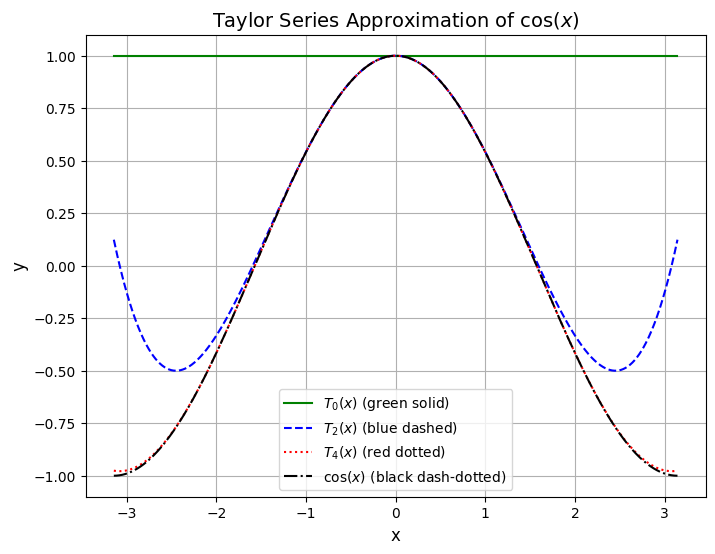
\includegraphics[width=0.75\linewidth]{AMath301/image2.png}
\end{figure}

\item [3. ]
The given function is:
\[
f(x) = x^3 - x^2 + 2x + 3
\]
with initial guess \( x_0 = -1 \). We aim to perform two iterations of the Newton-Raphson method using the formula:
\[
x_{n+1} = x_n - \frac{f(x_n)}{f'(x_n)}
\]

Computing \( f'(x) \)
The derivative of \( f(x) \) is:
\[
f'(x) = 3x^2 - 2x + 2
\]

Iteration 1: Starting with \( x_0 = -1 \)

First, calculate \( f(x_0) \) and \( f'(x_0) \):
\[
f(x_0) = (-1)^3 - (-1)^2 + 2(-1) + 3 = -1 - 1 - 2 + 3 = -1
\]
\[
f'(x_0) = 3(-1)^2 - 2(-1) + 2 = 3 + 2 + 2 = 7
\]

Using the Newton-Raphson formula:
\[
x_1 = x_0 - \frac{f(x_0)}{f'(x_0)} = -1 - \frac{-1}{7} = -1 + \frac{1}{7} = -\frac{6}{7}
\]

Iteration 2: Using \( x_1 = -\frac{6}{7} \)

First, calculate \( f(x_1) \):
\[
f(x_1) = \left(-\frac{6}{7}\right)^3 - \left(-\frac{6}{7}\right)^2 + 2\left(-\frac{6}{7}\right) + 3
\]
Compute each term:
\[
\left(-\frac{6}{7}\right)^3 = -\frac{216}{343}, \quad \left(-\frac{6}{7}\right)^2 = \frac{36}{49}, \quad 2\left(-\frac{6}{7}\right) = -\frac{12}{7}
\]
Substitute back:
\[
f(x_1) = -\frac{216}{343} - \frac{36}{49} - \frac{12}{7} + 3
\]
Convert to a common denominator of 343:
\[
f(x_1) = -\frac{216}{343} - \frac{252}{343} - \frac{588}{343} + \frac{1029}{343}
\]
\[
f(x_1) = \frac{-216 - 252 - 588 + 1029}{343} = \frac{-27}{343}
\]

Next, calculate \( f'(x_1) \):
\[
f'(x_1) = 3\left(-\frac{6}{7}\right)^2 - 2\left(-\frac{6}{7}\right) + 2
\]
\[
f'(x_1) = 3\left(\frac{36}{49}\right) + \frac{12}{7} + 2
\]
\[
f'(x_1) = \frac{108}{49} + \frac{84}{49} + \frac{98}{49} = \frac{290}{49}
\]

Finally, calculating \( x_2 \):
\[
x_2 = x_1 - \frac{f(x_1)}{f'(x_1)} = -\frac{6}{7} - \frac{\frac{-27}{343}}{\frac{290}{49}}
\]
Simplifing:
\[
\frac{\frac{-27}{343}}{\frac{290}{49}} = \frac{-27}{343} \times \frac{49}{290} = \frac{-27 \times 49}{343 \times 290} = \frac{-1323}{99570}
\]
\[
x_2 = -\frac{6}{7} + \frac{1323}{99570} = -\frac{6 \times 14265}{99570} + \frac{1323}{99570}
\]
\[
x_2 = \frac{-85590 + 1323}{99570} = \frac{-84267}{99570}
\]

The two iterations yield:
\[
x_1 = -\frac{6}{7}, \quad x_2 = \frac{-84267}{99570}
\]

PS: Did i have to use so many fractions to get the answer? It seems excessive.
\item [4.]
The function is:
\[
f(x) = \log_2(x) + x,
\]


The initial guesses are \( x_0 = 2 \) and \( x_1 = 1 \).

First, calculate \( f(x_0) \) and \( f(x_1) \):
\[
f(x_0) = \log_2(2) + 2 = 1 + 2 = 3,
\]
\[
f(x_1) = \log_2(1) + 1 = 0 + 1 = 1.
\]

Now, perform the first iteration (\( n = 1 \)) using the formula:
\[
x_2 = x_1 - f(x_1) \cdot \frac{x_1 - x_0}{f(x_1) - f(x_0)}.
\]
Substitute the values:
\[
x_2 = 1 - 1 \cdot \frac{1 - 2}{1 - 3},
\]
\[
x_2 = 1 - 1 \cdot \frac{-1}{-2},
\]
\[
x_2 = 1 - \frac{1}{2} = \frac{1}{2}.
\]

Next, calculate \( f(x_2) \):
\[
f\left(\frac{1}{2}\right) = \log_2\left(\frac{1}{2}\right) + \frac{1}{2},
\]
\[
\log_2\left(\frac{1}{2}\right) = \frac{\ln\left(\frac{1}{2}\right)}{\ln(2)} = \frac{-\ln(2)}{\ln(2)} = -1,
\]
\[
f\left(\frac{1}{2}\right) = -1 + \frac{1}{2} = -\frac{1}{2}.
\]

For the second iteration (\( n = 2 \)):
\[
x_3 = x_2 - f(x_2) \cdot \frac{x_2 - x_1}{f(x_2) - f(x_1)}.
\]
Substitute the values:
\[
x_3 = \frac{1}{2} - \left(-\frac{1}{2}\right) \cdot \frac{\frac{1}{2} - 1}{-\frac{1}{2} - 1},
\]
\[
x_3 = \frac{1}{2} - \left(-\frac{1}{2}\right) \cdot \frac{-\frac{1}{2}}{-\frac{3}{2}},
\]
\[
x_3 = \frac{1}{2} - \left(-\frac{1}{2}\right) \cdot \frac{1}{3},
\]
\[
x_3 = \frac{1}{2} + \frac{1}{6} = \frac{3}{6} + \frac{1}{6} = \frac{4}{6} = \frac{2}{3}.
\]

After two iterations of the Secant method:
\[
x_2 = \frac{1}{2}, \quad x_3 = \frac{2}{3}.
\]

\end{enumerate}

\end{document}
